% =============================================================================
% mpi_learning_material.tex
% Learning Material: MPI Distributed-Memory Parallelism
% EC7207 High Performance Computing – Group 11
% =============================================================================
\documentclass[12pt,a4paper]{article}

\usepackage[margin=2.5cm]{geometry}
\usepackage{listings}
\usepackage{xcolor}
\usepackage{amsmath}
\usepackage{booktabs}
\usepackage{hyperref}
\usepackage{tikz}
\usepackage{array}
\usepackage{enumitem}
\usepackage{fancyhdr}
\usepackage{titlesec}

\lstdefinestyle{cstyle}{
    language=C,
    basicstyle=\ttfamily\small,
    keywordstyle=\color{blue}\bfseries,
    commentstyle=\color{gray}\itshape,
    stringstyle=\color{red!70!black},
    numbers=left, numberstyle=\tiny\color{gray},
    numbersep=8pt, frame=single, rulecolor=\color{black!30},
    breaklines=true, showstringspaces=false,
    backgroundcolor=\color{gray!5},
    tabsize=4
}
\lstset{style=cstyle}

\pagestyle{fancy}
\fancyhf{}
\lhead{EC7207 HPC – Group 11}
\rhead{MPI — Distributed-Memory Parallelism}
\cfoot{\thepage}

\titleformat{\section}{\large\bfseries}{}{0em}{}[\titlerule]
\titleformat{\subsection}{\normalsize\bfseries}{}{0em}{}

% =============================================================================
\begin{document}
% =============================================================================

\begin{center}
    {\LARGE\bfseries MPI — Message Passing Interface}\\[0.3em]
    {\large Distributed-Memory Parallelism}\\[0.5em]
    {\large Learning Material for EC7207 High Performance Computing}\\[0.3em]
    {\normalsize Group 11 — Pearson Correlation Recommender System}
\end{center}
\vspace{1em}\hrule\vspace{1.5em}

% =============================================================================
\section{What is MPI?}
% =============================================================================

\textbf{MPI (Message Passing Interface)} is the industry standard for
distributed-memory parallel programming.  It enables programs to run across
multiple processes that each have their own \textbf{private address space} —
unlike OpenMP/Pthreads where all threads share the same RAM.

\subsection{The Fundamental Difference: Private Memory Spaces}

\begin{center}
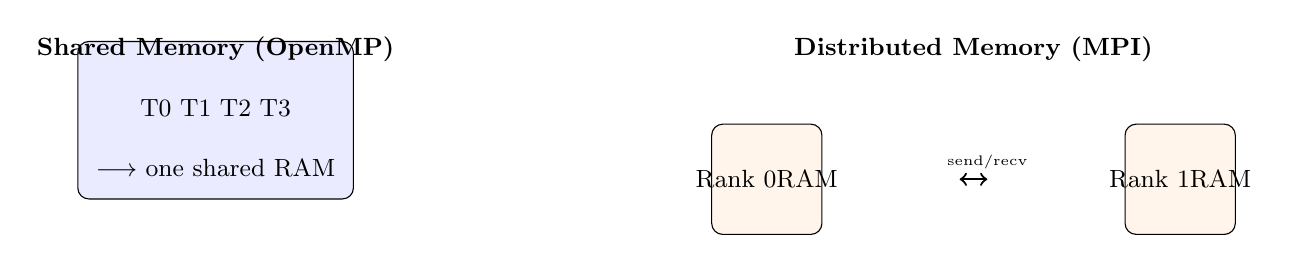
\begin{tikzpicture}[x=3.5cm,y=1.5cm]
    % Shared memory (OpenMP)
    \node[draw,rounded corners,fill=blue!8,minimum width=3.5cm,
          minimum height=2cm] at (0,0) {};
    \node[font=\small\bfseries] at (0,0.6) {Shared Memory (OpenMP)};
    \node[font=\small] at (0,0.1) {T0 T1 T2 T3};
    \node[font=\small] at (0,-0.4) {$\longrightarrow$ one shared RAM};

    % Distributed memory (MPI)
    \node[draw,rounded corners,fill=orange!8,minimum width=1.4cm,
          minimum height=1.4cm] at (2,-0.5) {};
    \node[draw,rounded corners,fill=orange!8,minimum width=1.4cm,
          minimum height=1.4cm] at (3.5,-0.5) {};
    \node[font=\small\bfseries] at (2.75,0.6) {Distributed Memory (MPI)};
    \node[font=\small] at (2,-0.5) {Rank 0\\RAM};
    \node[font=\small] at (3.5,-0.5) {Rank 1\\RAM};
    \draw[<->,thick] (2.7,-0.5) -- (2.8,-0.5) node[above,font=\tiny]{send/recv};
\end{tikzpicture}
\end{center}

\begin{itemize}
    \item Each MPI \textbf{rank} (process) is an independent program copy with
          its own private memory.
    \item Data cannot be read from another rank by dereferencing a pointer —
          it must be \textbf{explicitly sent} using MPI calls.
    \item \texttt{mpirun -np 4} launches 4 independent copies of the
          executable.  Each learns its rank number and total count via
          \texttt{MPI\_Comm\_rank()} and \texttt{MPI\_Comm\_size()}.
\end{itemize}

\subsection{Why MPI?}

\begin{itemize}
    \item \textbf{Scalability}: MPI programs can run across thousands of compute
          nodes (each with their own RAM and CPU) connected by a network.
          OpenMP is limited to one shared-memory machine.
    \item \textbf{HPC clusters}: real supercomputers are built from many nodes;
          MPI is how they are programmed.
    \item \textbf{Memory per node}: if the problem doesn't fit in one node's RAM,
          distributing it across nodes is the only option.
\end{itemize}

% =============================================================================
\section{MPI Initialisation and Finalisation}
% =============================================================================

\begin{lstlisting}
#include <mpi.h>

int main(int argc, char *argv[])
{
    /* MUST be the first MPI call in the program */
    MPI_Init(&argc, &argv);

    int mpi_rank, mpi_size;
    MPI_Comm_rank(MPI_COMM_WORLD, &mpi_rank); /* "what is my rank?" */
    MPI_Comm_size(MPI_COMM_WORLD, &mpi_size); /* "how many total?" */

    /* ... all program logic here ... */

    /* MUST be the last MPI call */
    MPI_Finalize();
    return 0;
}
\end{lstlisting}

\begin{itemize}
    \item \texttt{MPI\_COMM\_WORLD} = the default communicator containing
          every rank in the job.  A communicator defines a group of ranks
          that can communicate with each other.
    \item Rank 0 is conventionally the ``master'' that handles I/O.
    \item \textbf{Important}: \texttt{MPI\_Finalize()} must be called by
          \emph{all} ranks.  If one rank exits early without calling it, the
          other ranks may hang forever waiting for a collective operation.
\end{itemize}

% =============================================================================
\section{Row Partitioning Strategy}
% =============================================================================

Our strategy is \textbf{row partitioning}: divide the $N_{\text{USERS}}$ rows
of the ratings and similarity matrices evenly across ranks.

\begin{lstlisting}
static void get_range(int rank, int size, int *start, int *end)
{
    int chunk = (N_USERS + size - 1) / size;  /* ceiling division */
    *start = rank * chunk;
    *end   = *start + chunk;
    if (*end > N_USERS) *end = N_USERS;
}
\end{lstlisting}

\textbf{Example} ($N = 1000$, 4 ranks):
\begin{center}
\begin{tabular}{clll}
\toprule
Rank & start & end & Rows owned \\
\midrule
0 & 0   & 250 & 0--249 \\
1 & 250 & 500 & 250--499 \\
2 & 500 & 750 & 500--749 \\
3 & 750 & 1000 & 750--999 \\
\bottomrule
\end{tabular}
\end{center}

% =============================================================================
\section{Data Generation: No Communication Needed}
% =============================================================================

\begin{lstlisting}
/* All ranks call srand(SEED=42) and execute identical rand() sequences */
static void generate_data(void)
{
    srand(SEED);
    /* ... same three-dice process as serial version ... */
    if (mpi_rank == 0)   /* only rank 0 prints to avoid N duplicate lines */
        printf("[Data]   Users: ...\n");
}
\end{lstlisting}

\textbf{Key insight:}  Because C's \texttt{rand()} is a deterministic
algorithm seeded with a fixed value, all ranks produce \emph{identical}
ratings matrices without any communication.  This avoids broadcasting a
large array across the network — much cheaper.

% =============================================================================
\section{Collective Operation 1: \texttt{MPI\_Allgatherv}}
% =============================================================================

\subsection{Concept}

\texttt{MPI\_Allgatherv} collects pieces from all ranks and distributes the
complete assembled result back to \emph{every} rank (not just rank 0).

\begin{center}
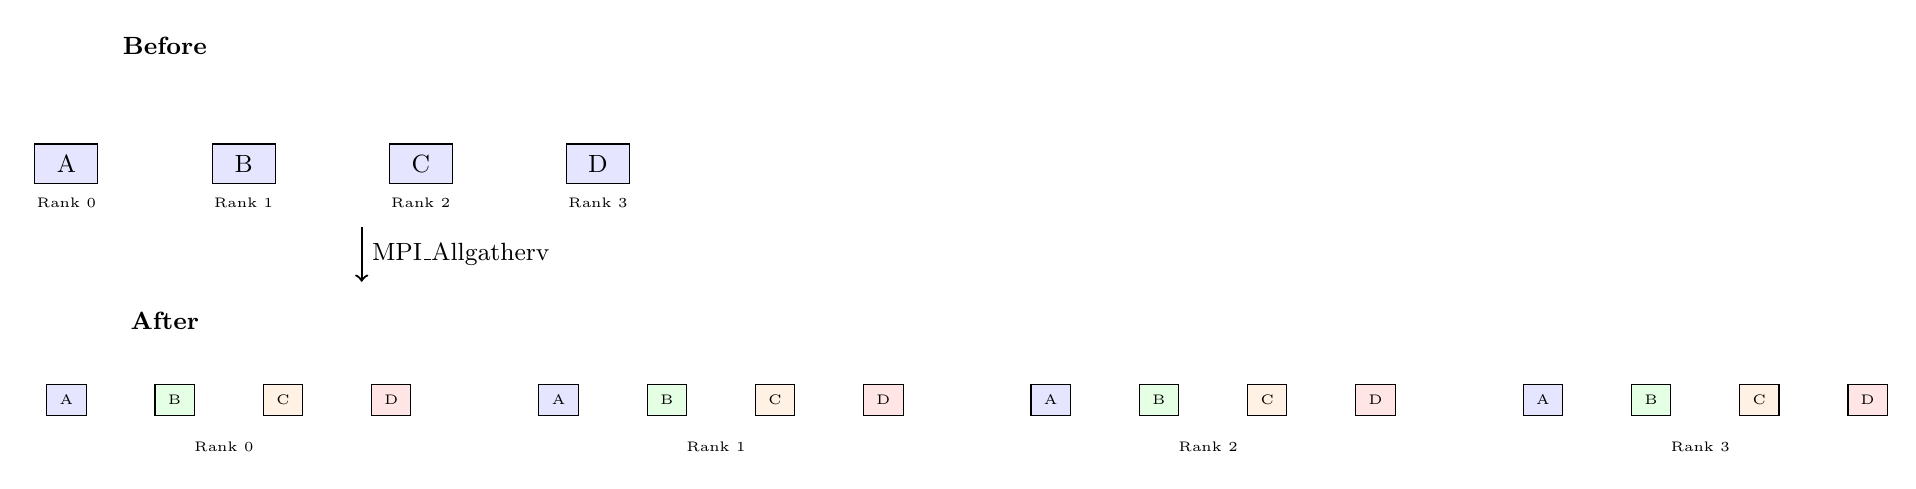
\begin{tikzpicture}[x=2.5cm,y=1cm]
    % Before
    \node[font=\small\bfseries] at (0.5,1.5) {Before};
    \foreach \r/\d in {0/A,1/B,2/C,3/D} {
        \node[draw,minimum width=0.8cm,minimum height=0.5cm,fill=blue!10,font=\small]
              at (\r*0.9,0) {\d};
        \node[font=\tiny] at (\r*0.9,-0.5) {Rank \r};
    }
    % Arrow
    \draw[->,thick] (1.5,-0.8) -- (1.5,-1.5)
        node[midway,right,font=\small]{MPI\_Allgatherv};
    % After
    \node[font=\small\bfseries] at (0.5,-2) {After};
    \foreach \r in {0,1,2,3} {
        \foreach \col/\d/\c in {0/A/blue,1/B/green,2/C/orange,3/D/red} {
            \node[draw,minimum width=0.5cm,minimum height=0.4cm,
                  fill=\c!10,font=\tiny]
                  at (\r*2.5+\col*0.55,-3) {\d};
        }
        \node[font=\tiny] at (\r*2.5+0.8,-3.6) {Rank \r};
    }
\end{tikzpicture}
\end{center}

\subsection{Parameters}

\begin{lstlisting}
MPI_Allgatherv(
    &user_mean[start_u],  /* sendbuf: my slice of the array   */
    end_u - start_u,      /* sendcount: floats I contribute    */
    MPI_FLOAT,            /* datatype                          */
    user_mean,            /* recvbuf: full destination array   */
    recvcounts,           /* int[]: floats from each rank      */
    displs,               /* int[]: offset in recvbuf per rank */
    MPI_FLOAT,
    MPI_COMM_WORLD
);
\end{lstlisting}

\subsection{recvcounts and displs Arrays}

These two arrays describe how the receive buffer is partitioned:

\begin{lstlisting}
/* Built once in main() for user_mean (1 float per user) */
for (int r = 0; r < mpi_size; r++) {
    int s, e;
    get_range(r, mpi_size, &s, &e);
    mean_recvcounts[r] = e - s;  /* how many floats rank r sends */
    mean_displs[r]     = s;      /* where in recvbuf to place them */
}

/* For sim_matrix (N_USERS floats per row): scale by N_USERS */
sim_recvcounts[r] = (e - s) * N_USERS;
sim_displs[r]     = s * N_USERS;
\end{lstlisting}

After \texttt{MPI\_Allgatherv}, every rank has a complete, identical copy
of \texttt{user\_mean[]} (or \texttt{sim\_matrix[]}).

% =============================================================================
\section{Collective Operation 2: \texttt{MPI\_Reduce}}
% =============================================================================

\texttt{MPI\_Reduce} combines one value from each rank into a single result
on one rank (the ``root''):

\begin{lstlisting}
/* Each rank computes its partial error over test entries it owns */
double local_err = 0.0;
int    local_cnt = 0;
for (int t = 0; t < test_size; t++) {
    int u = test_set[t].user;
    if (u < start_u || u >= end_u) continue;  /* not my user */
    local_err += fabs(PRED(u, ...) - test_set[t].rating);
    local_cnt++;
}

/* Sum all local_err values to rank 0 */
double global_err = 0.0;
int    global_cnt = 0;
MPI_Reduce(&local_err, &global_err, 1, MPI_DOUBLE, MPI_SUM, 0, MPI_COMM_WORLD);
MPI_Reduce(&local_cnt, &global_cnt, 1, MPI_INT,    MPI_SUM, 0, MPI_COMM_WORLD);

if (mpi_rank == 0)
    printf("[Eval] MAE = %.4f\n", global_err / global_cnt);
\end{lstlisting}

\textbf{Parameters of \texttt{MPI\_Reduce}:}
\begin{center}
\begin{tabular}{ll}
\toprule
Parameter & Meaning \\
\midrule
\texttt{sendbuf} & Local value to contribute \\
\texttt{recvbuf} & Where the result is stored (only meaningful on root) \\
\texttt{count} & Number of elements \\
\texttt{datatype} & \texttt{MPI\_DOUBLE}, \texttt{MPI\_INT}, \texttt{MPI\_FLOAT}, \ldots \\
\texttt{op} & Operation: \texttt{MPI\_SUM}, \texttt{MPI\_MAX}, \texttt{MPI\_MIN}, \ldots \\
\texttt{root} & The rank that receives the result \\
\bottomrule
\end{tabular}
\end{center}

% =============================================================================
\section{Synchronisation: \texttt{MPI\_Barrier}}
% =============================================================================

\begin{lstlisting}
MPI_Barrier(MPI_COMM_WORLD);  /* all ranks wait here */
t0 = MPI_Wtime();
compute_all_similarities(start_u, end_u, ...);
MPI_Barrier(MPI_COMM_WORLD);  /* all ranks done before measuring */
t1 = MPI_Wtime() - t0;
\end{lstlisting}

\textbf{Why barrier around timed sections?}  Without the first barrier, some
ranks might have already started computing while slower ranks are still in
the previous phase.  Rank 0's timer would then undercount the true wall-clock
cost.  The barrier ensures all ranks start the phase together.

% =============================================================================
\section{Timing: \texttt{MPI\_Wtime()}}
% =============================================================================

\begin{lstlisting}
static inline double now_sec(void) { return MPI_Wtime(); }
\end{lstlisting}

\texttt{MPI\_Wtime()} returns seconds as a \texttt{double}.  It is:
\begin{itemize}
    \item Defined by the MPI standard — portable across all MPI implementations
    \item Monotonically increasing (never goes backwards)
    \item A wall-clock timer (measures elapsed time, not CPU time)
\end{itemize}

% =============================================================================
\section{MPI Parallelisation Strategy Per Phase}
% =============================================================================

\begin{center}
\begin{tabular}{lll}
\toprule
Phase & Strategy & Communication \\
\midrule
1. Data generation &
  All ranks run same \texttt{srand(42)} sequence &
  None \\
2. User means &
  Each rank computes its rows [start, end) &
  \texttt{MPI\_Allgatherv} assembles full array \\
3. Similarity &
  Each rank computes all columns for its rows &
  \texttt{MPI\_Allgatherv} assembles full matrix \\
4. Predictions &
  Each rank predicts for its users only &
  None (sim\_matrix already complete) \\
5. MAE &
  Each rank accumulates partial error &
  \texttt{MPI\_Reduce} sums to rank 0 \\
\bottomrule
\end{tabular}
\end{center}

\subsection{Why Full Rows (Not Upper Triangle) in Phase 3?}

In the serial/OpenMP versions, we use the upper triangle ($v > u$) and mirror.
In the MPI version, rank $r$ fills \emph{all columns} $v = 0, \ldots, N-1$
for its rows $u \in [\text{start}, \text{end})$.  Why?

\textbf{Reason}: With upper triangle, rank 0 would only have pairs where $v > u$
but not $v < u$ — the sendbuf for \texttt{MPI\_Allgatherv} would have ``holes.''
Computing all columns means each rank sends a contiguous block of exactly
$(\text{local\_rows} \times N_{\text{USERS}})$ floats — simple and correct.

The duplicate computation (SIM(u,v) and SIM(v,u) both computed by different ranks
for some pairs) is a deliberate trade-off: slight extra computation for much
simpler communication pattern.

% =============================================================================
\section{Error Handling in MPI: \texttt{MPI\_Abort}}
% =============================================================================

\begin{lstlisting}
if (!ratings || !user_mean ...) {
    fprintf(stderr, "Rank %d: memory allocation failed.\n", mpi_rank);
    MPI_Abort(MPI_COMM_WORLD, EXIT_FAILURE);
    /* terminates ALL ranks immediately */
}
\end{lstlisting}

\textbf{Why \texttt{MPI\_Abort} not \texttt{exit()}?}  If one rank calls
\texttt{exit()}, the other ranks continue running and may hang indefinitely
waiting for a collective operation that will never arrive (deadlock).
\texttt{MPI\_Abort} terminates all ranks in the communicator immediately.

% =============================================================================
\section{MPI Datatypes}
% =============================================================================

\begin{center}
\begin{tabular}{ll}
\toprule
C type & MPI type \\
\midrule
\texttt{int} & \texttt{MPI\_INT} \\
\texttt{float} & \texttt{MPI\_FLOAT} \\
\texttt{double} & \texttt{MPI\_DOUBLE} \\
\texttt{char} & \texttt{MPI\_CHAR} \\
Custom struct & \texttt{MPI\_Type\_create\_struct()} \\
\bottomrule
\end{tabular}
\end{center}

We use \texttt{MPI\_FLOAT} for user\_mean and sim\_matrix, and
\texttt{MPI\_DOUBLE} for the error accumulator.

% =============================================================================
\section{Performance Analysis}
% =============================================================================

\subsection{Communication Overhead}

The main communication bottleneck is the \texttt{MPI\_Allgatherv} for
\texttt{sim\_matrix}:

\[
\text{Data transferred per rank} = \text{local\_rows} \times N_{\text{USERS}} \times 4\,\text{bytes}
\]

For $N = 1000$, 4 ranks: each rank sends $250 \times 1000 \times 4 = 1\,\text{MB}$.
On a 10~Gbit/s InfiniBand network, this takes $\approx 1\,\text{ms}$ — negligible
compared to the computation ($\sim$seconds).

\subsection{Scalability}

\textbf{Strong scaling}: fixed problem size, increase process count.
Speedup should approach $p$ (linear), limited by:
\begin{itemize}
    \item Communication cost (grows logarithmically for collective operations)
    \item Load imbalance (last rank may have fewer rows)
    \item Serial fractions (Phase 1)
\end{itemize}

\textbf{Weak scaling}: increase problem size proportionally with process count
(keep work per process constant).  Ideal: constant runtime.  Deviation
reveals communication overhead scaling.

% =============================================================================
\section{Compile and Run}
% =============================================================================

\begin{verbatim}
# Compile (mpicc wraps gcc with MPI include/library paths)
mpicc -O2 -Wall -o mpi_rec mpi/mpi_recommender.c -lm

# Run with different process counts
mpirun -np 1 ./mpi_rec 1000 1000    # 1 process (serial-equivalent)
mpirun -np 2 ./mpi_rec 1000 1000
mpirun -np 4 ./mpi_rec 1000 1000
mpirun -np 8 ./mpi_rec 1000 1000

# On a real cluster (SLURM):
# srun -n 4 ./mpi_rec 1000 1000
\end{verbatim}

% =============================================================================
\section{Key Points to Explain in a Presentation}
% =============================================================================

\begin{enumerate}
    \item \textbf{How is MPI different from OpenMP?}  MPI = separate processes
          with private memory + explicit messages.  OpenMP = threads with shared
          memory.  MPI scales to clusters; OpenMP is limited to one machine.
    \item \textbf{Why \texttt{MPI\_Allgatherv} and not \texttt{MPI\_Gather}?}
          \texttt{MPI\_Gather} puts the result only on rank 0.  Our Phase 4
          (predictions) needs the full sim\_matrix on \emph{every} rank so they
          can independently compute predictions without further communication.
    \item \textbf{Why does each rank generate its own data instead of rank 0
          generating and broadcasting?}  Cheaper and simpler.  All ranks produce
          identical data with \texttt{srand(42)}, so no network transfer is needed.
    \item \textbf{What is the \texttt{v} suffix in \texttt{MPI\_Allgatherv}?}
          The \texttt{v} means ``variable'' — different ranks contribute different
          \emph{amounts} of data.  Without it (\texttt{MPI\_Allgather}), all
          ranks must contribute exactly the same count.
    \item \textbf{What happens at the end?}  Only rank 0 prints results (to
          avoid $N$ duplicate lines).  All ranks must call \texttt{MPI\_Finalize()}
          before any rank can exit.
\end{enumerate}

\vfill
\begin{center}
    \small\textit{Group 11 — EC7207 High Performance Computing}
\end{center}

\end{document}
